Um die Winkelrichtgröße nach Formel \eqref{eqn:D} berechnen zu können, werden
die Daten aus Tabelle \ref{MessD} benötigt.
\begin{table}[H]
  \centering
  \begin{tabular}{c c c}
    \toprule
    $\varphi$ & F & r \\
    Grad & $\si{\milli\newton}$ & $\si{\meter}$ \\
    \midrule
    30  &    15   &   0.27  \\
    30  &    55   &   0.15  \\
    40  &    78   &   0.15  \\
    50  &   108   &   0.15  \\
    30  &    39   &   0.19  \\
    10  &    43   &   0.04  \\
    30  &    90   &   0.10  \\
    20  &    48   &   0.08  \\
    60  &    57   &   0.28  \\
    50  &    75   &   0.18  \\
    \bottomrule
  \end{tabular}
  \caption{Messdaten zur Bestimmung von D}
  \label{MessD}
\end{table}
Der Wert für den Winkel wird noch mit der Formel
\begin{equation*}
  \varphi_\su{rad}\frac{\varphi}{360}\cdot2\pi
\end{equation*}
umgerechnet. Nachdem $D$ für die verschiedenen Werte berechnet wurde, wird der
Mittelwert berechnet und der Fehler bestimmt. Somit erhält man für die
Winkelrichtgrße einen Wert von
\begin{equation*}
  D= (0.014 \pm 0.003) \,\si{\newton\meter}.
\end{equation*}
\begin{table}
  \centering
  \begin{tabular}{c c c}
    \toprule
    $\varphi$ & a & T \\
    Grad & \cm & \sek \\
    \midrule
    50    &    8  &   2.96    \\
    50    &   10  &   3.44    \\
    50    &   12  &   3.77    \\
    50    &   14  &   4.29    \\
    50    &   16  &   4.77    \\
    50    &   18  &   5.11    \\
    50    &   20  &   5.55    \\
    50    &   22  &   6.05    \\
    50    &   24  &   6.71    \\
    50    &   26  &   7.22    \\
    50    &   28  &   7.71    \\
    \bottomrule
  \end{tabular}
  \caption{Messwerte zur Bestimmung von $I_\su{D}$}
  \label{messI}
\end{table}
Anschließend wird das Eigenträgheitsmoment der Feder der Apparatur bestimmt,
indem mit den Werten aus Tabelle \ref{messI} ein Graph erstellt wird, bei dem
$T^2$ gegen $a^2$ aufgetragen wird. Abbildung \ref{fig:trag} zeigt diesen Graph.
\begin{figure}[H]
  \centering
  \includegraphics[width=0.8\textwidth]{bilder/tragheit.pdf}
  \caption{Graph zur Bestimmung des Eigenträgheitsmoments}
  \label{fig:trag}
\end{figure}
Mit Hilfe der linearen Regression lässt sich das $I_\su{D}$ nun einfach bestimmen.
Die mit Python 3.5.2 berechneten Werte lauten
\begin{align*}
  a &= (1.42 \pm 0.02)\,\cdot10^{-3} \\
  b &= (6.0 \pm 0.8)\,\cdot10^{-3}.
\end{align*}
Der Parameter a ist hierbei der gesuchte Wert für die Eigenträgheit.
Als nächstes werden die Trägheitsmomente von einem aufrechten und einem liegenden
Zylinder gemessen und mit den theoretischen Werten verglichen. Die Abmessungen
der beiden Zylinder sind mit einer Höhe von $3\cm$ und einem Durchmesser von $7.5\cm$
gleich. Somit unterscheiden sie sich lediglich im Gewicht. Der Aufrechte Zylinder
wiegt $1119.3\gr$ und das Gewicht des liegenden Zylinders liegt bei $1117.3\gr$.
Um das Trägheitsmoment bestimmen zu können, werden beide Körper jeweils 5 Mal um
50° ausgelenkt. Die gemittelten Periodenschwingsdauern betragen
\begin{align*}
  T_\su{a} &= (0.97 \pm 0.02)\sek \\
  T_\su{l} &= (0.82 \pm 0.04)\sek.
\end{align*}
Das Trägheitsmoment lässt sich nun mittels einer Umformung von Formel \eqref{eqn:T}
berechnen. Die Formel für den Fehler ergibt sich aus der Gaußschen Fehlerfortpflanzung
und lautet:
\begin{equation*}
  \Delta I = \sqrt{\biggl(\frac{2TD}{4\pi^2}\biggr)^2\cdot\sigma_\su{T}^2 +
  \biggl(\frac{T^2}{4\pi^2}\biggr)^2\cdot\sigma_\su{D}^2}
\end{equation*}
Somit betragen die experimentell festgestellten Werte für die Trägheitsmomente
der Zylinder
\begin{align*}
  T_\su{a} &= (3.4 \pm 0.8)\,\cdot10^{-4}\,\si{\kilo\gram\square\meter} \\
  T_\su{l} &= (2.4 \pm 0.9)\,\cdot10^{-4}\,\si{\kilo\gram\square\meter}.
\end{align*}
Die theoretischen Werte lassen sich mit Formel \eqref{eqn:ZylI} berechnen.
Da der Durchmesser und die Höhe der Zylinder eindeutig bestimmt werden können,
bleibt eine Fehlerrechnung aus.
Die theoretischen Werte lauten:
\begin{align}
  T_\su{a} &= 7.9\,\cdot10^{-4}\,\si{\kilo\gram\square\meter} \\
  T_\su{l} &= 4.8\,\cdot10^{-4}\,\si{\kilo\gram\square\meter}.
\end{align}

% Puppe
Bei der ersten Stellung der Puppe werden die Arme als Zylinder angenommen, die sich um
ihre Querachse drehen und ihren Ansatz im Mittelpunkt der Drehachse haben. Somit werden
ihre Trägheitsmomente mit dem Satz von Steiner um $\sfrac{l_\su{arm}}{2}$ verschoben.
Die restlichen Körperteiler werden als Zylinder angenommen, die sich um ihre Symmetrieachse
drehen und sich im Mittelpunkt der Drehachse befinden.
In der zweiten Stellung wird zusätzlich angenommen, dass sich auch die Beine um ihre
Querachse drehen. Auch ihr Trägheitsmoment wird mittels Steiner um $\sfrac{l_\su{bein}}{2}$
verschoben. Die Stellungen sind in Abbildung \ref{fig:stellung} zu sehen.
\begin{figure}
  \centering
  \begin{subfigure}{0.48\textwidth}
    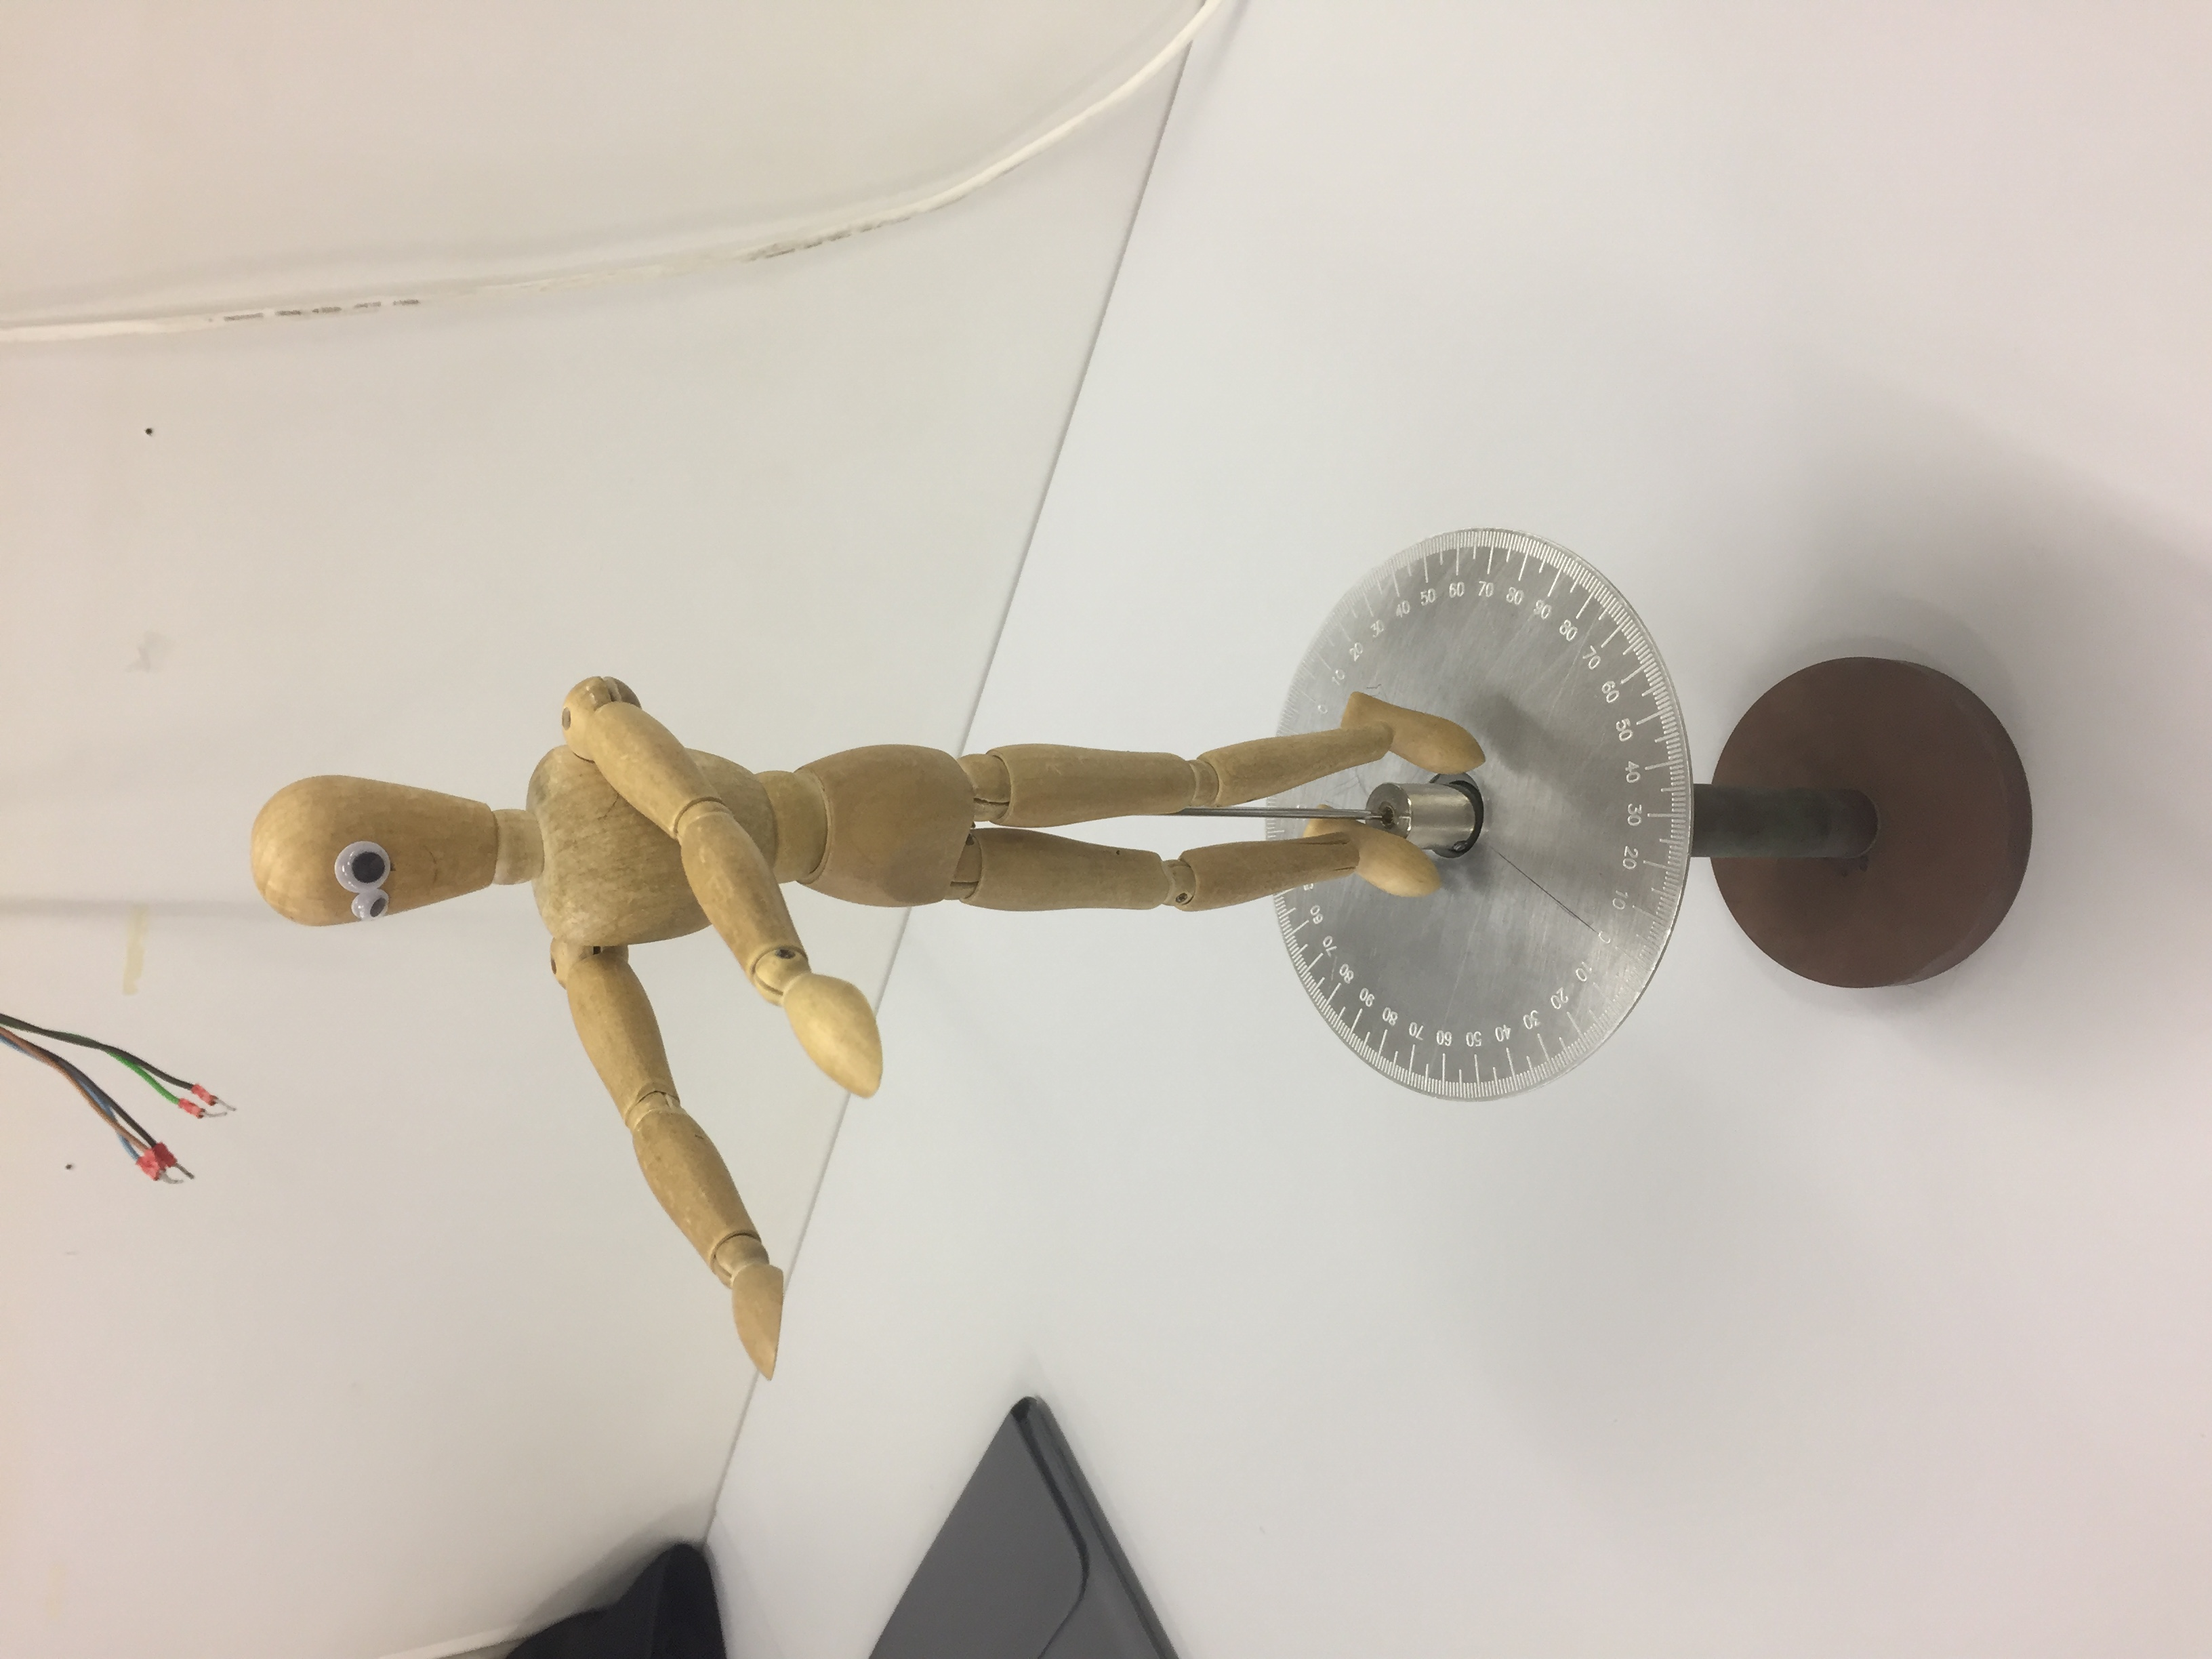
\includegraphics[width=5cm]{bilder/stellung1.JPG}
  \end{subfigure}
  \begin{subfigure}{0.48\textwidth}
    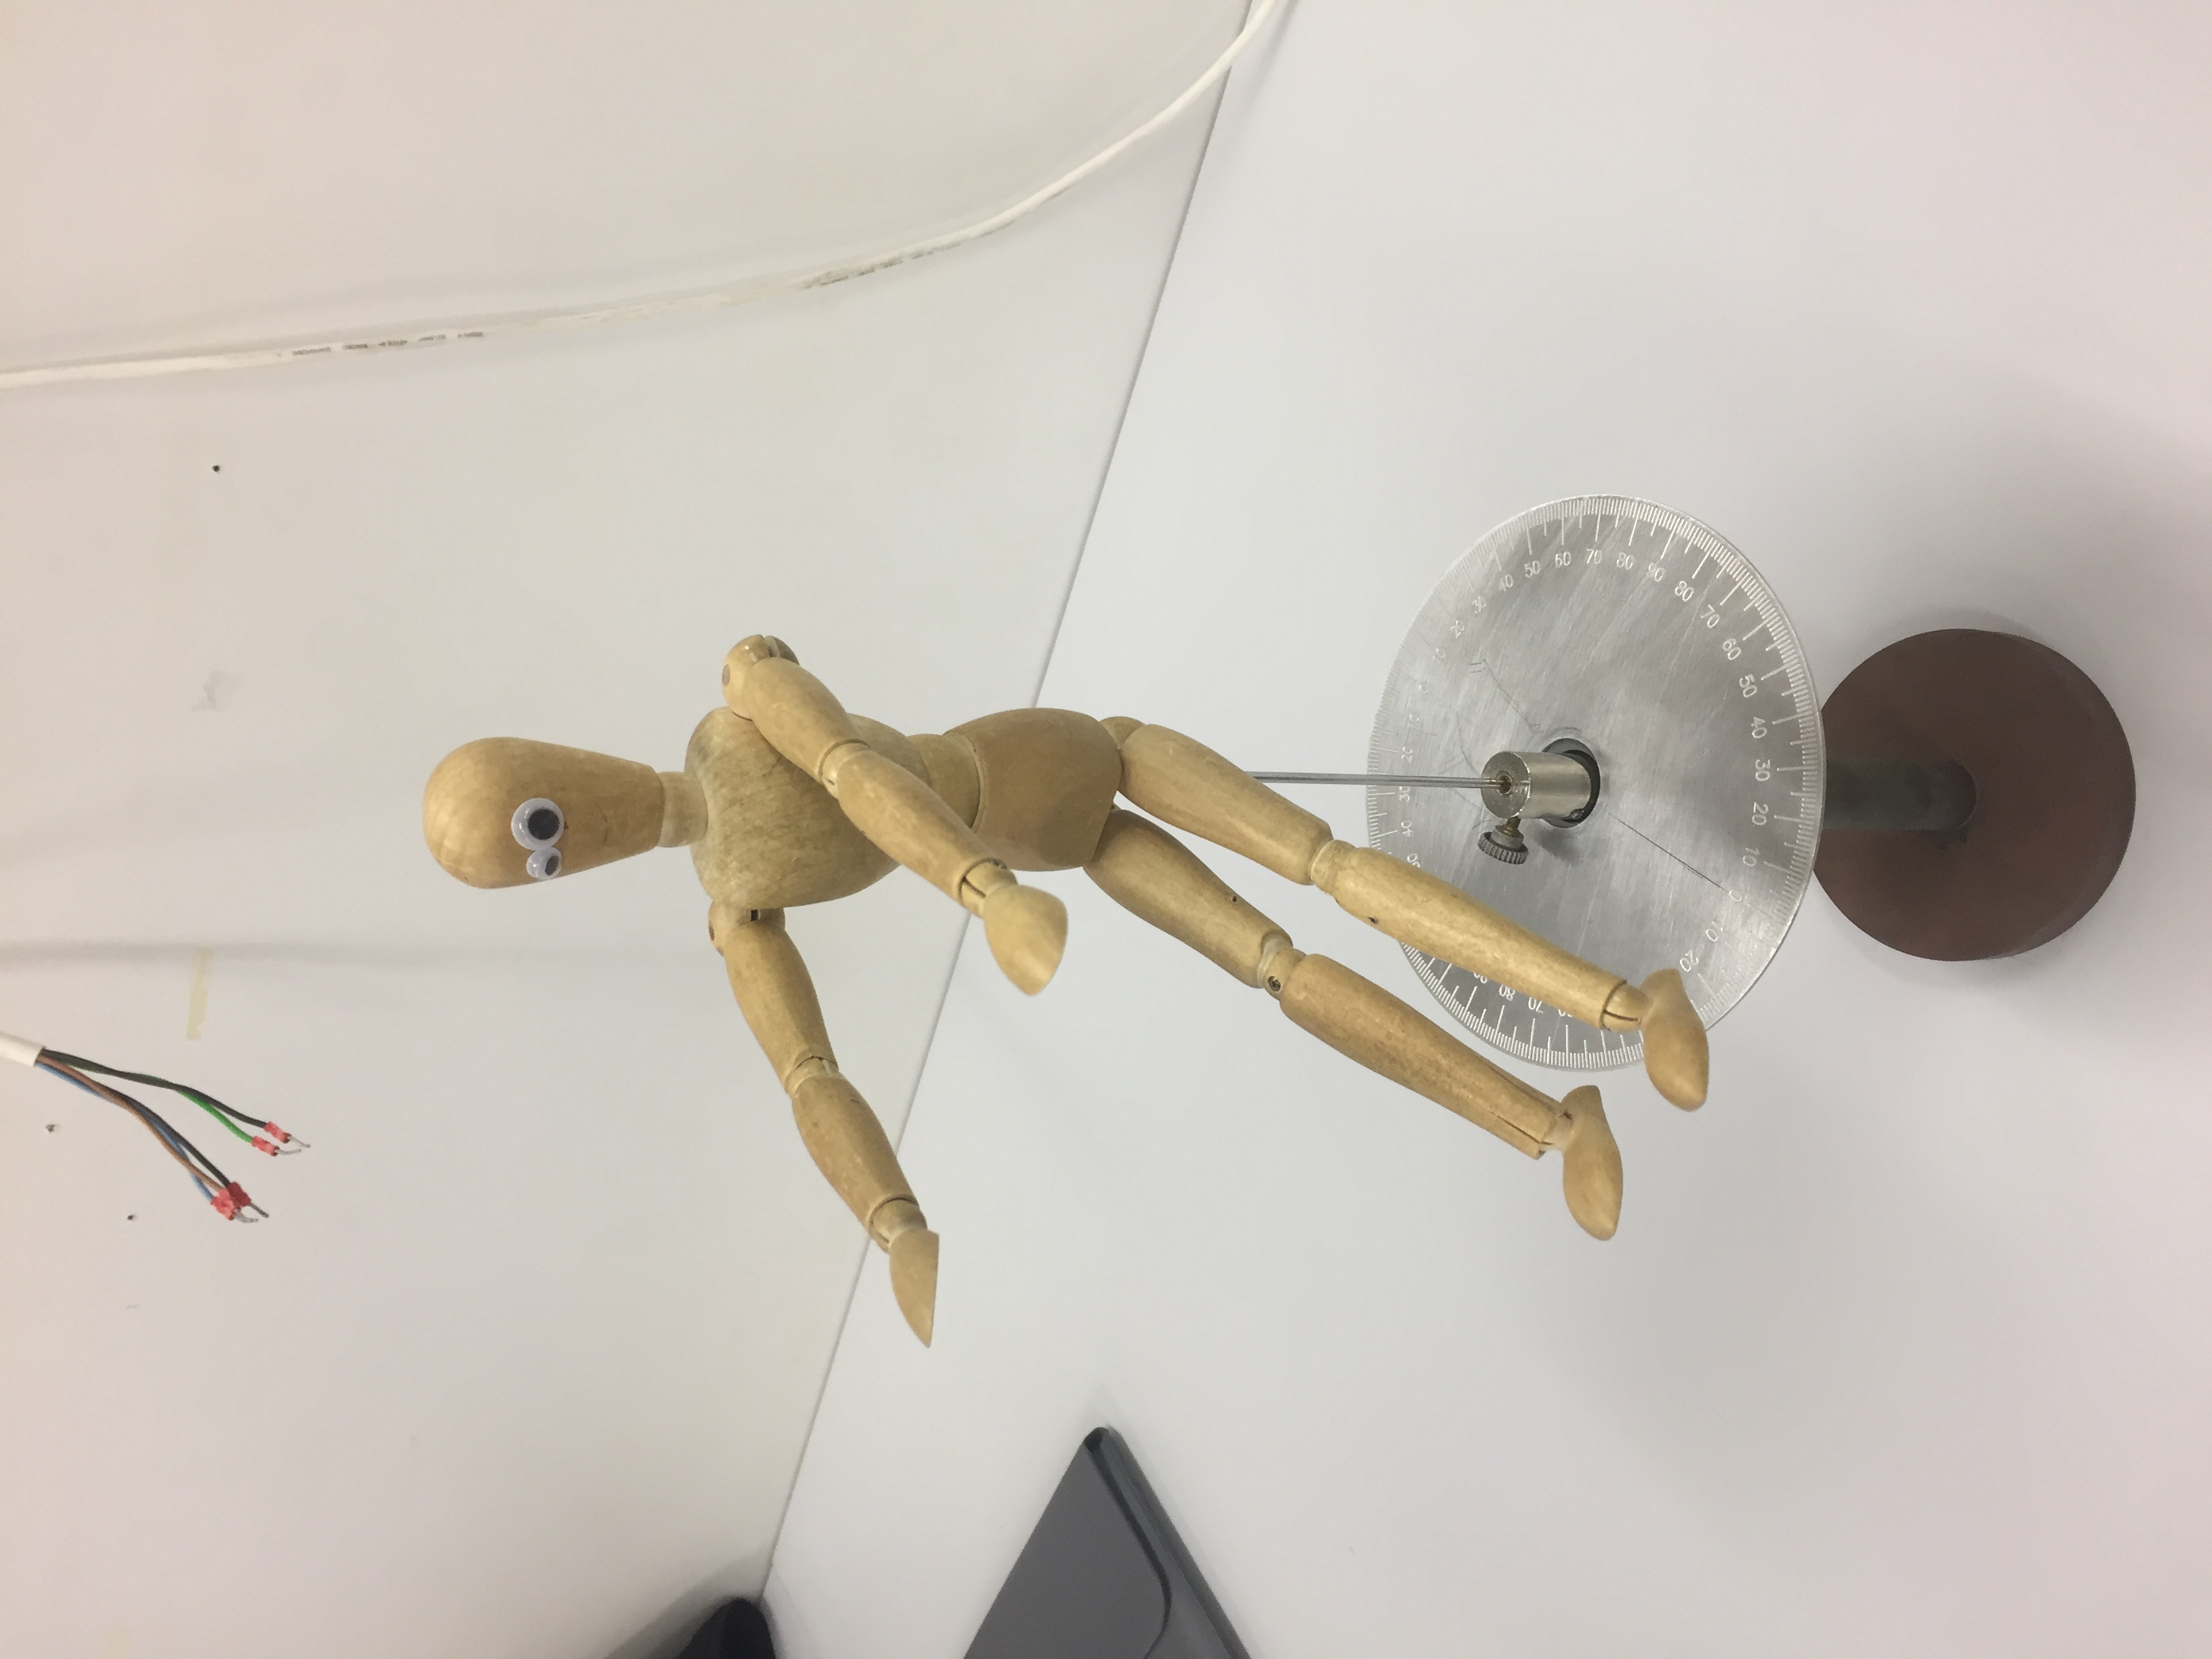
\includegraphics[width=5cm]{bilder/stellung2.JPG}
  \end{subfigure}
  \caption{Die 2 Stellungen der Puppe}
  \label{fig:stellung}
\end{figure}
Die Maße der Zylinder ergeben sich aus den Mittelwerten der verschiedenen Messungen.
Der Werte sind in Tabelle \ref{tab:wertepuppe} einzusehen.
\begin{table}
  \centering
  \begin{tabular}{c c c c}
    \toprule
    $\su{Zylinder}$ & $d \,/\,\cm$ & $l\,/\,\cm$ & $ m\,/\,\si{\gram}$ \\
    \midrule
    Kopf & 2.5±0.5 & 5.54±0.05 & 48.69 \\
    Bein & 1.5±0.3 & 16.3±0.8 & 16.93 \\
    Rumpf & 3.6±0.6 & 9.70±0.09 & 56.28 \\
    Arm & 1.3±0.2 & 14.2±0.1 & 11.14 \\
    \bottomrule
  \end{tabular}
  \caption{Maße der Zylinder von der Puppe}
  \label{tab:wertepuppe}
\end{table}
Die gesamte Puppe wiegt $m = 161.1\,\si{\gram}$. Um auf die Gewichte der einzelnen
Körperteile zu kommen wird die Dichte der Puppe mittels
\begin{equation}
  \rho = \frac{m}{V}
\end{equation}
bestimmt. Die Volumina der Zylinder errechnen sich mittels
\begin{equation}
  V = \pi r^2 \cdot l.
\end{equation}
Für das gesamte Volumen folgt $V = 0.28893 \cum$. Damit ergibt sich für die
Dichte $ \rho = 557.57 \,\si{\gram\per\cubic\meter}$. Die Massen sind
in Tabelle \ref{tab:wertepuppe} zu finden.

Die Trägheitsmomente um die Symmetrieachse werden alle nach
\begin{equation}
  I_\su{sym} = \frac{mr^2}{2}
\end{equation}
bestimmt.
Für die Trägheitsmomente um die Querachse, welche zusätzlich verschoben sind,
wird die Formel
\begin{equation}
  I_\su{quer,steiner} = \frac{mr^2}{4} + \frac{ml^2}{12} + m \biggl(\frac{l}{2}\biggr)^2
\end{equation}
benutzt.
Für Stellung 1 ergibt sich damit das Trägheitsmoment
\begin{align}
  I_1 &= I_\su{Kopf} + I_\su{Rumpf} + 2 \cdot I_\su{Bein} + 2 \cdot I_\su{Arm,quer,steiner} \\
  I_1 &= 1.64 \cdot 10^{-4} \,\si{\kilo\gram\square\meter}
\end{align}
und für Stellung 2 ergibt sich das Trägheitsmoment
\begin{align}
  I_2 &= I_\su{Kopf} + I_\su{Rumpf} + 2 \cdot I_\su{Bein,quer,steiner} + 2 \cdot I_\su{Arm,quer,steiner} \\
  I_2 &= 4.64 \cdot 10^{-4} \,\si{\kilo\gram\square\meter}.
\end{align}
